В \textbf{главе 4} поднимается вопрос об универсальности полученных при исследовании модельного порыва результатов. Для установления универсальности рассчитаны и исследованы другие, отличные от модельного порыва, решения уравнений Навье-Стокса. В частности, исследованы условно-периодические решения уравнений Навье-Стокса с пространственно локализованной структурой, полученные продолжением решения, соответствующего модельному порыву, по параметру. Также исследовано три семейства решений, имеющих вид бегущей волны. Одно описывает течение в круглой трубе, два других --- в плоском канале. Все исследованные решения воспроизводят общий механизм поддержания колебаний, что подкрепляет представление о его универсальности.

\begin{figure}
\center{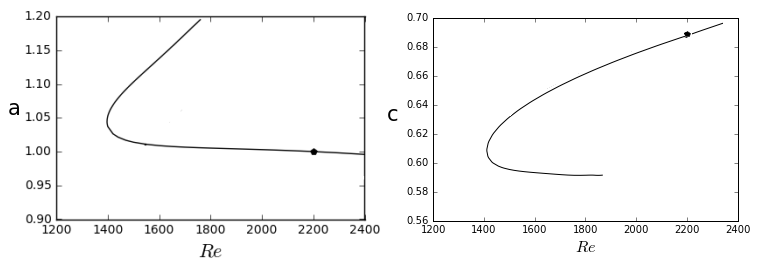
\includegraphics[width=0.9\linewidth]{autoref_contin.png}}
\caption{Продолжение модельного порыва по числу Рейнольдса}
\label{contin_pic}
\end{figure} 

В \textbf{разделе 4.1} описан метод Ньютона, позволивший найти новые условно-периодические решения уравнений Навье-Стокса и решения в виде бегущей волны, как частный случай условно-периодических. Приближение к решению возникающей на каждой итерации метода Ньютона линейной системы ищется в подпространствах Крылова методом минимизации невязки. %Поиск приближения к решению в подпространствах Крылова позволяет существенно снизить требования к вычислительным ресурсам, необходимым для применения метода Ньютона. 
Метод продолжения по параметру основан на применении метода Ньютона. Когда одно решение известно, оно используется в качестве начального приближения к решению при близком значении параметров, с которыми метод Ньютона сходится. Затем найденное решение используется в качестве начального приближения к новому решению, и т.д. Таким образом строятся цепочки решений, связывающие решения с существенно различными значениями параметров, --- исходное решение продолжается по параметру.


В \textbf{разделе 4.2} приведены результаты продолжения модельного порыва по числу Рейнольдса. Продолжение модельного порыва по $\Re$ позволило получить новые условно периодические решения уравнений Навье-Стокса с пространственно локализованной структурой. Решение в процессе продолжения определяется значением $\Re$ однозначно. Значения амплитуды трехмерной составляющей движения $a$ и скорости перемещения вдоль трубы $c$ как функции $\Re$ приведены на рисунке \ref{contin_pic}. Решения принадлежат однопараметрическому множеству. Жирные точки на графиках соответствуют исходному решению. При $\Re \approx 1400$ обнаружена точка бифуркации. При меньших $\Re$ решений не существует. При больших $\Re$ существует две ветви решений, то есть при каждом значении $\Re$ существует два решения, каждое из которых принадлежит свой ветви. Ветвь, которой принадлежит исходное решение, называют нижней. Вторую ветвь называют верхней. Для верхней ветви характера большая интенсивность пульсаций и меньшая скорость перемещения вдоль трубы. По этим и другим параметрам решения с верхней ветви приближаются к турбулентному порву. Результаты согласуются с (Avila et al. 2013). 

\begin{figure}
\center{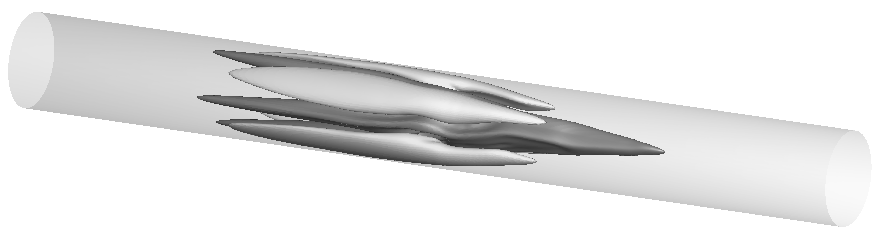
\includegraphics[width=0.9\linewidth]{autoref_3D_ub.png}}
\caption{Условно-периодическое решение с верхней ветви}
\label{3D_ub_pic}
\end{figure} 

В \textbf{разделе 4.3} выполнено исследование верхней ветви порожденного модельным порывом семейства условно-периодических решений. На рисунке \ref{3D_ub_pic} приведена визуализация мгновенного поля скорости решения с верхней ветви. Несмотря на существенные количественные отличия, решения с верхней ветви воспроизводят тот же механизм поддержания колебаний, что и решение с нижней ветви. Поле скорости решения представляется в виде суперпозиции средней и пульсационной составляющих. Области повышенной и пониженной средней скорости представляют собой вытянутые вдоль потока полосы. На рисунке \ref{ub_cs_pic}(a) приведены изолинии средней продольной скорости в поперечном сечении трубы, в котором пульсации имеют существенную амплитуду. В центральной части расчетной области, где изолинии находятся на большем удалении от стенки, проходит полоса пониженной скорости. При больших и меньших значениях $\theta$ находятся полосы повышенной скорости. Пульсации возникают в результате линейной неустойчивости среднего течения между соседними полосами повышенной и пониженной скорости. Угловую неоднородность среднего течения поддерживают продольные вихри, которым соответствуют области повышенных и пониженных значений средней продольной завихренности $\Omega_x$. Распределение $\Omega^2_x$ в том же сечении трубы приведено на рисунке \ref{ub_cs_pic}(б). Определяющий вклад в производство $\Omega_x$ в уравнении \eqref{OX_eq} дают слагаемые \eqref{OXgen_terms}. Вклад слагаемых, соответствующих \eqref{OXgen_terms}, в производство $\Omega^2_x$ приведен на рисунке \ref{ub_cs_pic}(в). Механизм образования пульсаций продольной завихренности в области формирования продольных вихрей также аналогичен выделенному в модельном порыве. 


\begin{figure}
\center{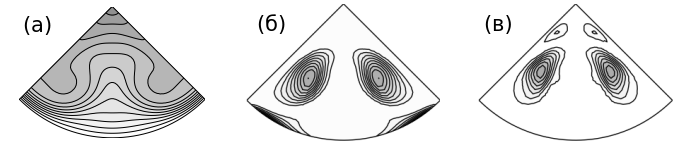
\includegraphics[width=0.9\linewidth]{ub_cs.png}}
\caption{Поле скорости решения с верхней ветви}
\label{ub_cs_pic}
\end{figure} 


\textbf{Разделы 4.4} и \textbf{4.5} посвящены анализу трехмерных бегущей волн в течении Гагена-Пуазейля и в плоском течении Пуазейля. Постановка задачи для плоского течения Пуазейля аналогична постановке для течение Гагена-Пуазейля. В каждом из двух течения вид бегущей волны имеют предельные решения на сепаратрисе, найденные в непротяженной расчетной области. Также в плоском течении Пуазейля при наложенных условиях симметрии существует устойчивая бегущая волна, найденная прямым интегрированием уравнений движения по времени. Методом продолжения по параметру рассчитаны соответствующие семейства решений. В отличии от модельного порыва, среднее поле скорости бегущей волны не зависит от продольной координаты --- полосы и продольные вихри имеют бесконечную протяженность. Решения достаточно существенно отличаются друг от друга, но несмотря на это, механизм поддержания колебаний во всех трех семействах решений аналогичен механизму поддержания колебаний в модельном порыве. Отметим, что в некоторых решениях среднее поле скорости устойчиво к малым возмущениям, но и в этих случаях механизм передачи энергии в пульсационную составляющую движения, по-видимому, линейный, так как наиболее медленно затухающая собственная функция линейной задачи устойчивости повторяет форму и фазовую скорость пульсационной составляющей движения. Также в некоторых решениях слагаемое \eqref{ox1gen_main_terms} оказывается не единственным, ответственным за производство $\omega'_x$ в области формирования продольных вихрей, но это слагаемое всегда имеет существенно значение и именно оно обеспечивает необходимую для поддержания продольных вихрей согласованность фаз между пульсациями $\omega'_x$ и $v'_x$. 

В \textbf{разделе 4.6} приведены выводы по главе. Основные результаты, приведенные в главе, опубликованы в работах автора диссертации \cite{Vest18, KMU2016}. 


